\chapter{Metaphern für Bitcoins Zukunft}
\label{les:21}

\begin{chapquote}{Lewis Carroll, \textit{Alice im Wunderland}}
\enquote{Ich weiß, dass sicher etwas interessantes passieren wird\ldots}
\end{chapquote}

In den letzten Jahrzehnten hat sich gezeigt, dass technologische Innovationen
keinem linearen Trend folgen. Egal, ob man an die technologische Singularität
glaubt oder nicht, es ist unbestreitbar, dass der Fortschritt in vielen
Bereichen exponentiell stattfindet. Aber nicht nur das, auch die
Geschwindigkeit mit der neue Technologien Anwendung finden, nimmt zu. Bevor man
sich versieht benützen unsere Kinder Snapchat anstatt hinter einem Busch
\enquote{ich zeig dir meines, du zeigst mir deines} zu spielen. Exponentielle
Kurven haben die Tendenz dir ins Gesicht zu schlagen, bevor du sie kommen
siehst.

Bitcoin ist eine exponentielle Technologie, die wiederum auf exponentiellen
Technologien basiert. \textit{Our World in
Data}\footnote{\url{https://ourworldindata.org/}} zeigt auf schöne Weise die
steigende Geschwindigkeit der technologischen Adaption, die 1903 mit der
Einführung des Festnetzes begann. Festnetz, Strom, Computer, Internet,
Smartphones; alle folgen exponentiellen Trends in Bezug auf Preis-Leistung und
Verwendung. Bitcoin tut das auch.

\begin{center}
  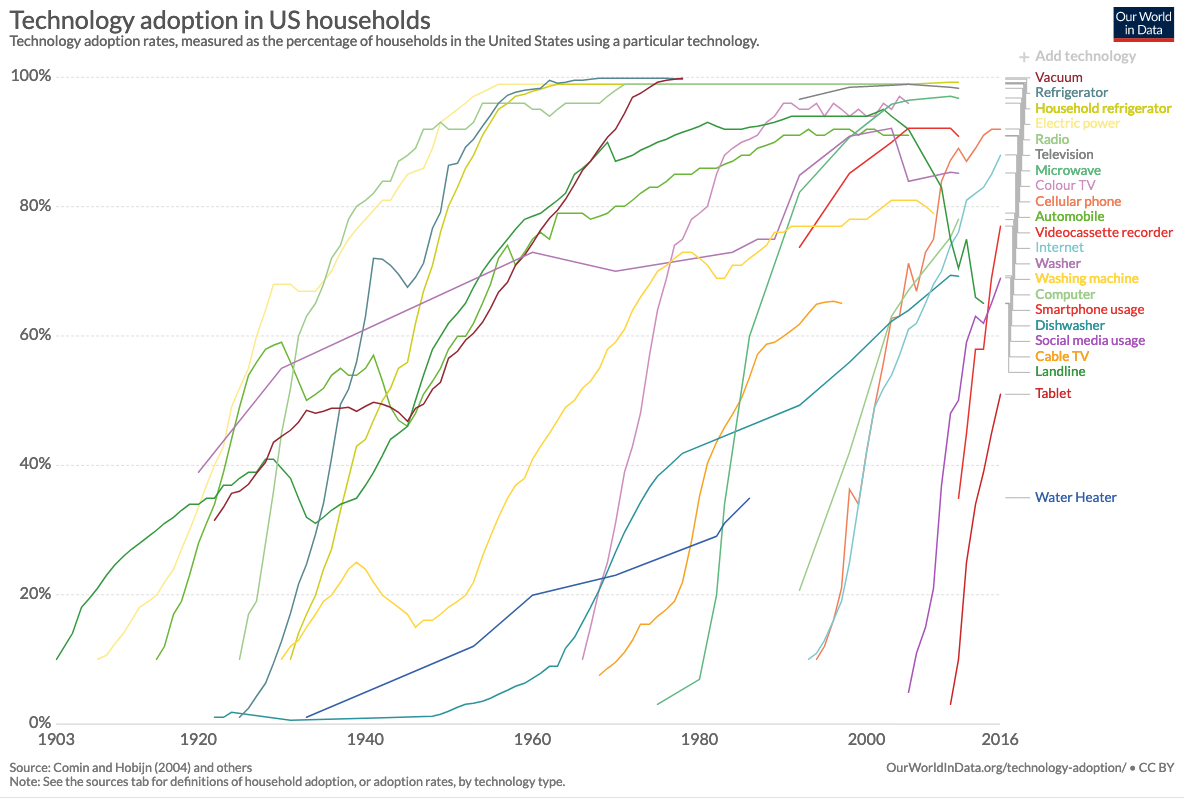
\includegraphics[width=\textwidth]{assets/images/tech-adoption.png}
  \captionof{figure}{Akzeptanzkurven verschiedener Technologien. Grafik cc-by Our World in Data}
  \label{fig:tech-adoption}
\end{center}

Bitcoin hat nicht nur einen, sondern mehrere Netzwerkeffekte\footnote{Trace
Mayer, \textit{The Seven Network Effects of Bitcoin} (\enquote{Die Sieben
Netzwerkeffekte von Bitcoin})~\cite{7-network-effects}}, die alle zu
exponentiellen Wachstumsmustern in ihrem jeweiligen Bereich führen: Preis,
Nutzer, Sicherheit, Entwickler, Marktanteil und Akzeptanz als globales Geld.

Nachdem Bitcoin seine Kindheit nun überstanden hat, entwickelt es sich jeden Tag
in mehrfacher Hinsicht weiter. Zugegeben, die Technologie ist noch nicht ganz
ausgereift. Wir befinden uns wahrscheinlich in Bitcoin's Pubertät. Aber wenn die
Technologie exponentiell ist, ist der Weg von Obskurität zu Ominpräsenz ein sehr
kurzer.

\begin{center}
  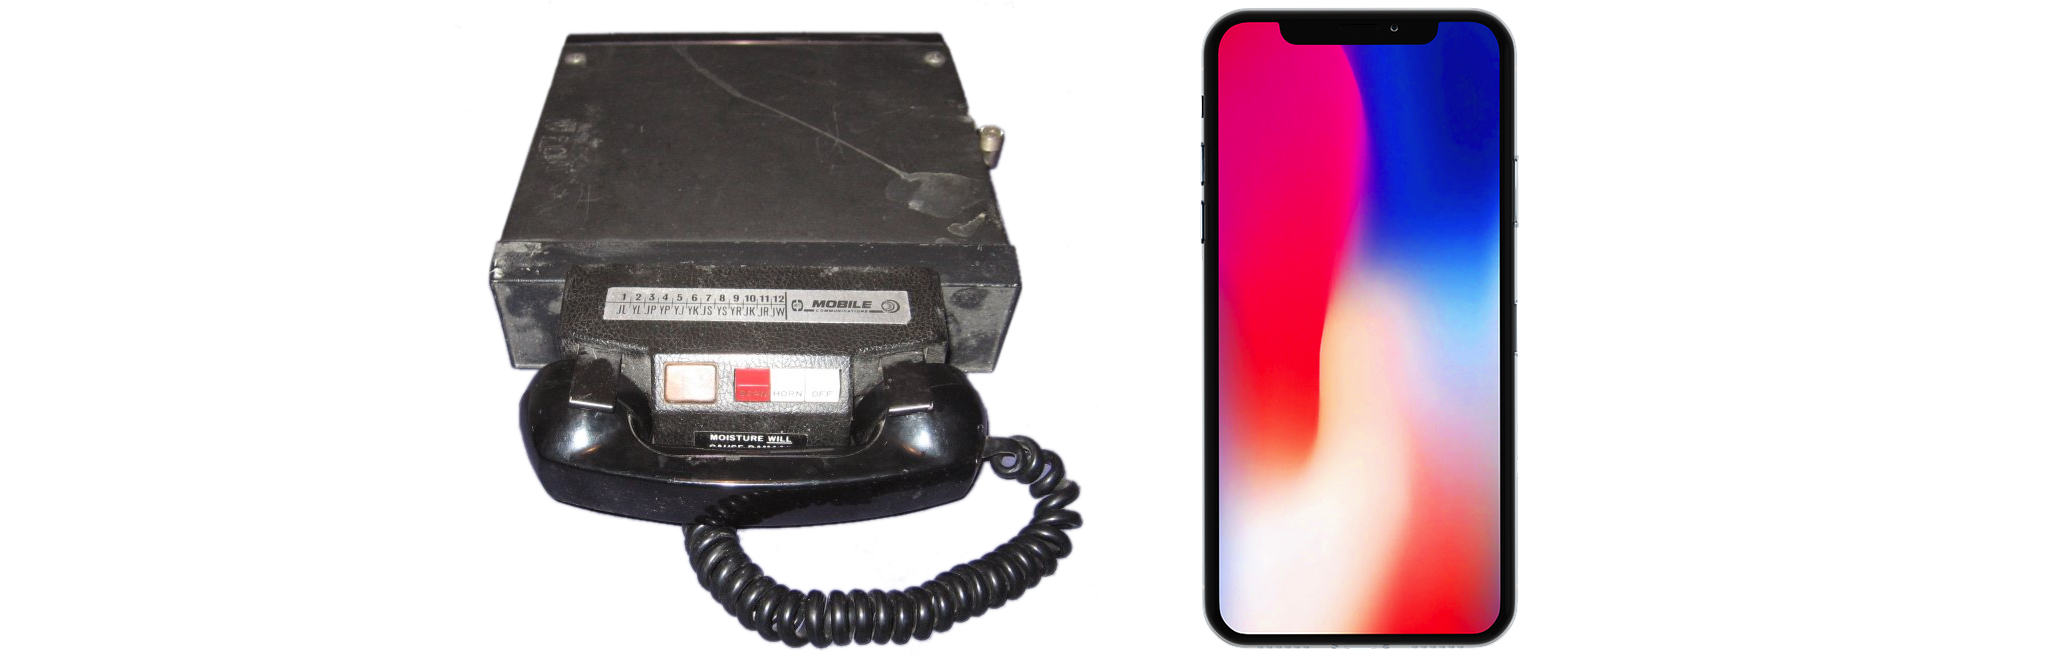
\includegraphics[width=\textwidth]{assets/images/mobile-phone.png}
  \captionof{figure}{Mobiltelefone, ca. 1965 vs 2019.}
  \label{fig:mobile-phone}
\end{center}

In seinem TED-Talk im Jahr 2003 entschied sich Jeff Bezos dafür, Strom als
Metapher für die Zukunft des Internets zu
verwenden.\footnote{\url{http://bit.ly/bezos-web}} Alle drei Phänomene ---
Elektrizität, Internet, Bitcoin --- sind Basistechnologien. Netzwerke, die
andere Dinge ermöglichen. Sie sind von fundamentaler Natur: Infrastruktur auf
der man aufbauen kann.

Elektrizität gibt es schon seit einiger Zeit. Wir nehmen sie als
selbstverständlich hin. Das Internet ist etwas jünger, aber die meisten Menschen
nehmen es auch schon länger als selbstverständlich hin. Bitcoin ist zehn Jahre
alt und hat mit dem Hype-Zyklus von 2017 die öffentliche Manege betreten. Nur
die frühesten Benutzer nehmen es als selbstverständlich hin. Mit zunehmender
Zeit werden immer mehr Menschen Bitcoin als etwas erkennen, das einfach nur
\enquote{ist}.\footnote{Dieser Effekt ist auch als \textit{Lindy-Effekt}
bekannt. Der Lindy-Effekt ist eine Theorie, welche besagt, dass die zukünftige
Lebenserwartung von nicht verderblichen Dingen (z.B. einer Technologie oder einer
Idee) proportional zu ihrem aktuellen Alter ist. Jede zusätzliche
Überlebensperiode impliziert eine längere verbleibende
Lebenserwartung.~\cite{wiki:lindy}}

Im Jahr 1994 war das Internet noch verwirrend und unintuitiv. Wenn man sich z.B.
eine alte Aufnahme der \textit{Today
Show}\footnote{\url{https://youtu.be/UlJku_CSyNg}} ansieht wird deutlich, dass
das, was sich heutzutage natürlich und intuitiv anfühlt, damals noch nicht
selbstverständlich war. Bitcoin ist immer noch verwirrend und den meisten fremd,
aber genau wie das Internet für \textit{Digital Natives} in Fleisch und Blut
übergeht, wird das Ausgeben und Horten von Satoshis (Stichwort:
\enquote{\textit{stacking
sats}}\footnote{\url{https://twitter.com/hashtag/stackingsats}}) eine
selbstverständliche Gewohnheit für die \textit{Bitcoin Natives} der Zukunft sein.

\begin{quotation}\begin{samepage}
\enquote{Die Zukunft ist bereits da -- sie ist nur nicht sehr gleichmäßig
verteilt.} \begin{flushright} -- William Gibson\footnote{William Gibson,
\textit{The Science in Science Fiction} \cite{william-gibson}}
\end{flushright}\end{samepage}\end{quotation}

Im Jahr 1995 nutzten etwa $15\%$ der amerikanischen Erwachsenen das Internet.
Historische Daten aus dem Pew Research Center~\cite{pew-research} zeigen, wie
sich das Internet in unser aller Leben verwoben hat. Laut einer
Verbraucherumfrage von Kaspersky Lab~\cite{web:kaspersky} haben $13\%$ der
Befragten Bitcoin und seine Klone verwendet, um 2018 für Waren zu bezahlen.
Obwohl Zahlungen nicht der einzige Anwendungsfall von Bitcoin sind, ist es ein
Hinweis darauf, wo wir uns in der Internetzeit befinden: Anfang bis Mitte der
90er Jahre.

1997 erklärte Jeff Bezos in einem Brief an seine Aktionäre~\cite{bezos-letter},
dass \enquote{dies der erste Tag für das Internet} sei und erkannte das große
ungenutzte Potenzial für das Internet und damit für sein Unternehmen. An welchem
Tag auch immer dies für Bitcoin geschieht, die riesigen Mengen an ungenutztem
Potenzial sind dann allen Leuten klar, selbst jenen Beobachtern die zur Zeit mit
wenig Interesse am Seitenrand stehen.

\begin{center}
  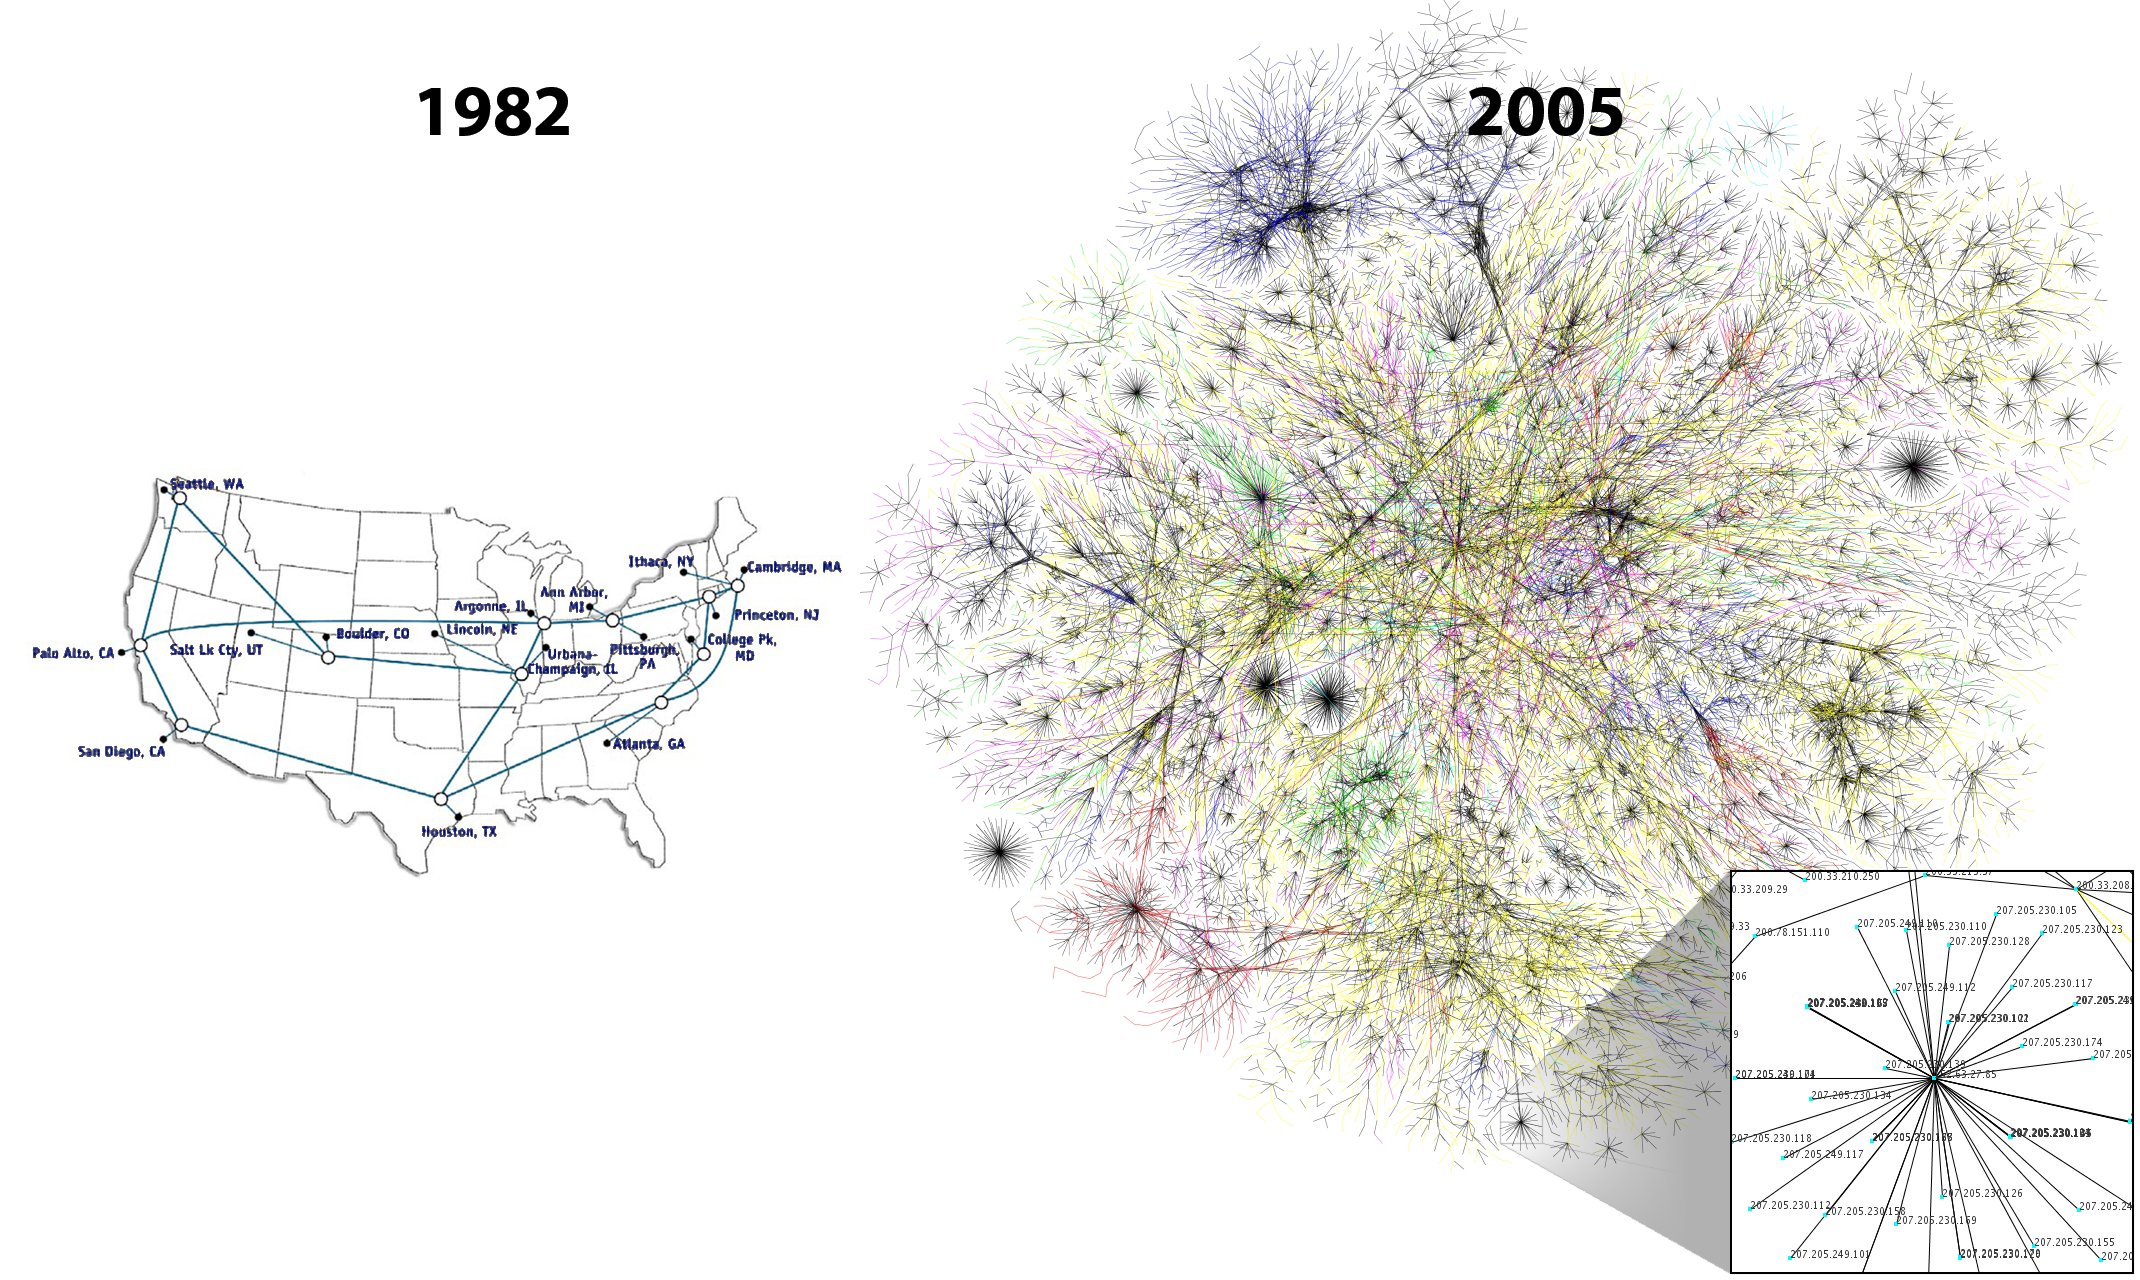
\includegraphics[width=\textwidth]{assets/images/internet-evolution-white-dates.png}
  \captionof{figure}{Das Internet, 1982 vs 2005. Quelle: cc-by Merit Network, Inc. und
  Barrett Lyon, Opte Project}
  \label{fig:internet-evolution-white-dates}
\end{center}

Der erste Knoten von Bitcoin ging 2009 online, nachdem Satoshi den
\textit{Genesis-Block}\footnote{ Der Genesis-Block ist der erste Block der
Bitcoin Blockchain. Moderne Versionen von Bitcoin nummerieren ihn als Block $0$,
obwohl sehr frühe Versionen ihn als Block $1$ zählten. Der Genesis-Block ist
normalerweise in der Software der Anwendungen, welche die Bitcoin Blockchain
verwenden, fest codiert.  Er ist ein Sonderfall, da er sich nicht auf einen
vorherigen Block bezieht und eine Subvention erzeugt, welche nicht ausgegeben
werden kann. Der \textit{Coinbase}-Parameter enthält neben den normalen Daten
den folgenden Text: \textit{\enquote{The Times 03/Jan/2009 Chancellor on brink
of second bailout for banks}} \cite{btcwiki:genesis-block}} geschürft und die
Software der Öffentlichkeit zugänglich gemacht hatte. Sein Knoten war nicht
lange allein. Hal Finney war einer der ersten der die Idee aufgriff und
sich dem Netzwerk anschloss. Zehn Jahre später, zum Zeitpunkt an dem ich diesen
Text verfasse, sind mehr als
$75.000$\footnote{\url{https://bit.ly/luke-nodecount}} Knoten mit dem Bitcoin
Netzwerk verbunden.

\begin{center}
  \centering
  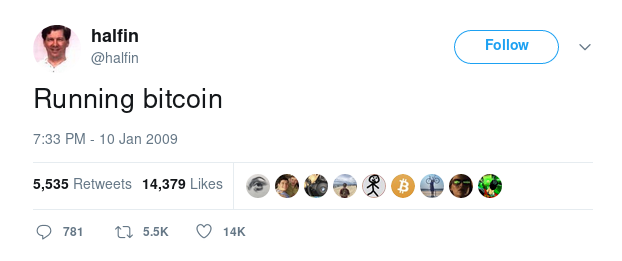
\includegraphics[width=8cm]{assets/images/running-bitcoin.png}
  \captionof{figure}{Hal Finney verfasste den ersten Tweet welcher Bitcoin erwähnte im
  Jänner 2009.}
  \label{fig:running-bitcoin}
\end{center}

Die Basisschicht des Protokolls ist nicht das Einzige was exponentiell wächst.
Das Lightning Netzwerk, eine Second-Layer-Technologie wächst sogar noch
schneller.

Im Januar 2018 hatte das Lightning-Netzwerk $40$ Knoten und $60$ Kanäle. Im
April 2019 wuchs das Netzwerk auf mehr als $4000$ Knoten und rund $40.000$
Kanäle. Man bedenke, dass es sich hierbei noch immer um eine experimentelle
Technologie handelt, bei der es zu Geldverlusten kommen kann und auch
tatsächlich kommt. Doch der Trend ist klar: Tausende von Menschen sind
\textit{\#reckless} (waghalsig) und brennen darauf die Technologie zu nutzen.

\begin{center}
  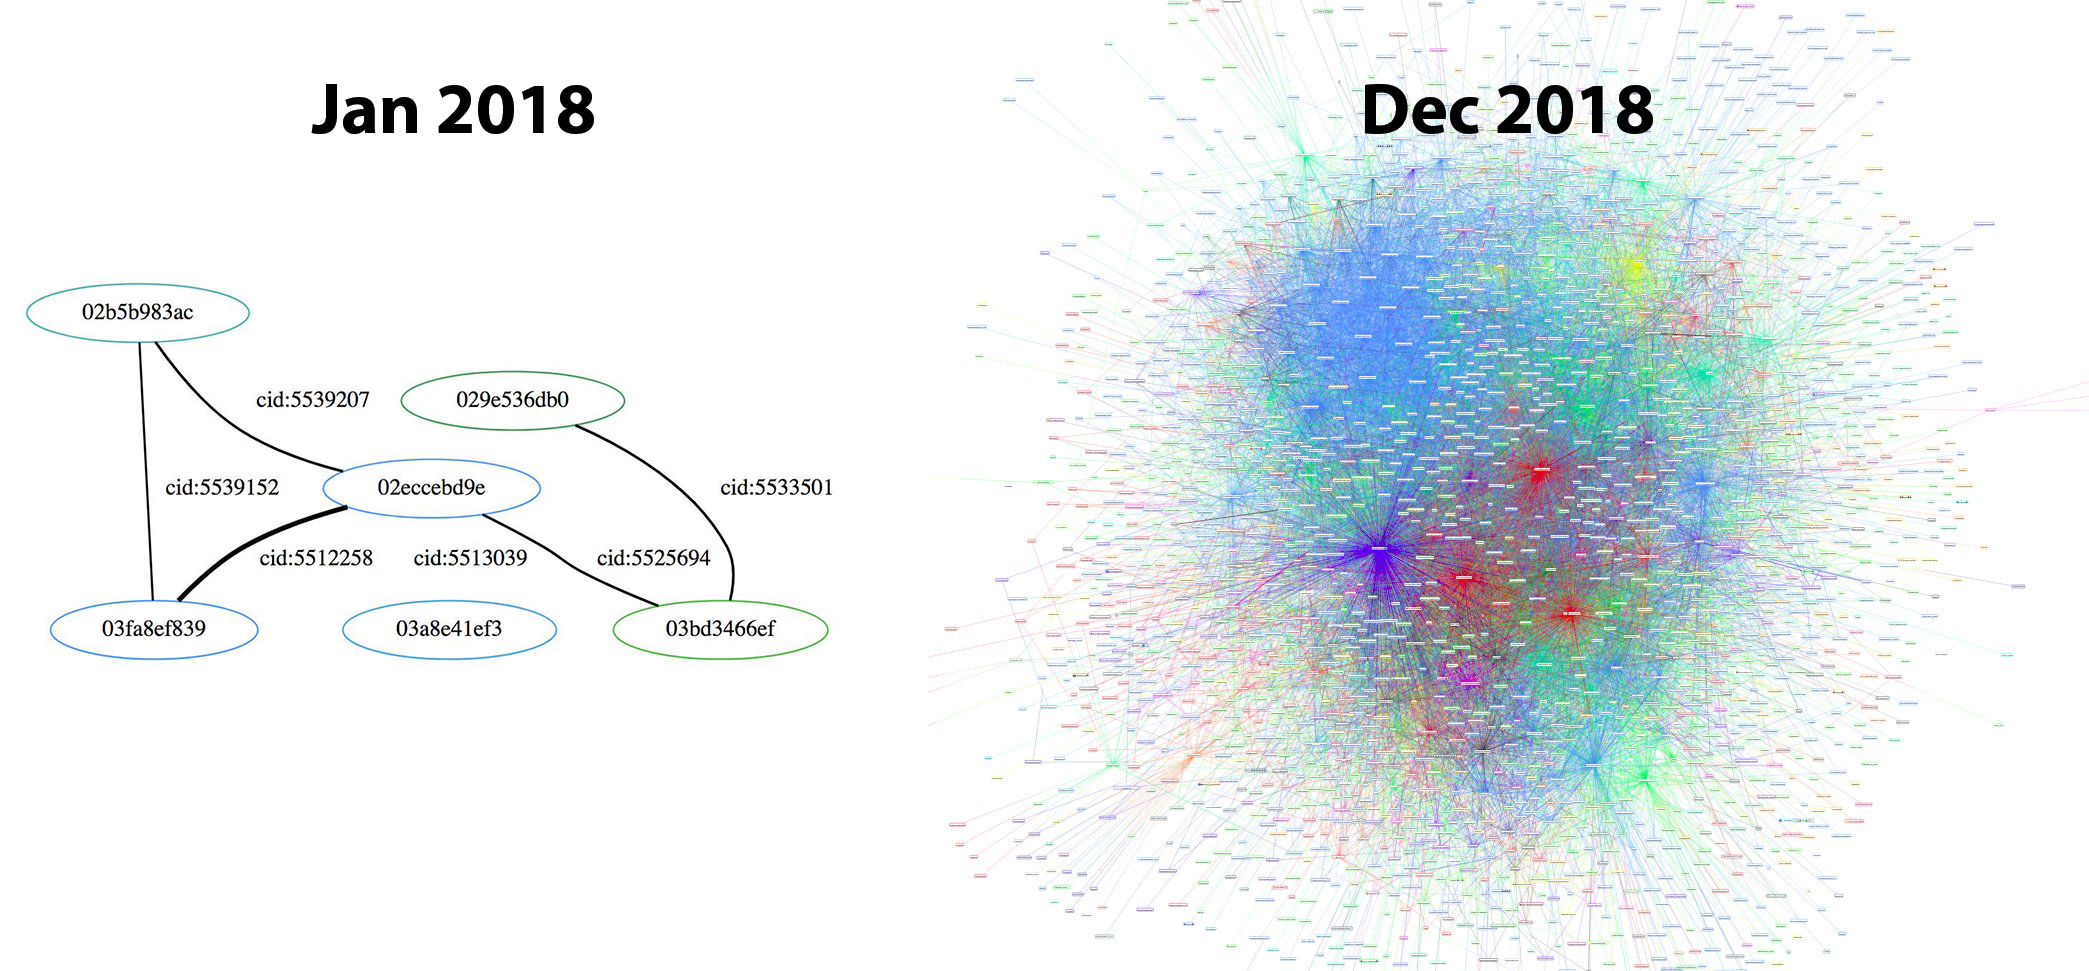
\includegraphics[width=\textwidth]{assets/images/lnd-growth-lopp-white.png}
  \captionof{figure}{Lightning Netzwerk, Jänner 2018 vs Dezember 2018. Quelle: Jameson Lopp}
  \label{fig:lnd-growth-lopp-white.png}
\end{center}

Für mich, als jemand der den rasanten Aufstieg des Internets miterlebt hat, sind
die Parallelen zwischen dem Internet und Bitcoin offensichtlich. Beide sind
Netzwerke, beide sind exponentielle Technologien und beide eröffnen neue
Möglichkeiten, neue Branchen, neue Lebensweisen. So wie Strom die beste Metapher
war, um zu verstehen in welche Richtung sich das Internet entwickeln wird,
könnte das Internet die beste Metapher sein um das Potential und die Zukunft von
Bitcoin zu verstehen. Oder, um es wie Andreas Antonopoulos ausdrücken: Bitcoin
ist das \textit{Internet des Geldes}. Diese Metaphern sind eine großartige
Möglichkeit sich zu vergegenwärtigen, dass sich die Geschichte zwar nicht
wiederholt, aber oft aufeinander reimt.

Exponentielle Technologien sind schwer zu erfassen und werden oft unterschätzt.
Auch wenn ich ein großes Interesse an solchen Technologien habe, bin ich immer
wieder überrascht vom Tempo des Fortschritts und der Innovation. Das Wachstum
des Bitcoin-Ökosystems zu beobachten ist wie den Aufstieg des Internets im
Schnelldurchlauf zu beobachten.

Meine intellektuelle Reise Bitcoin zu Verstehen hat mich auf mehr als eine Weise
auf die Pfade der Geschichte geführt. Das Verständnis alter gesellschaftlicher
Strukturen, vergangener Gelder und der Entwicklung von Kommunikationsnetzen war
Teil dieser Reise. Von der Handaxt bis zum Smartphone hat die Technologie
zweifellos unsere Welt um ein Vielfaches verändert. Vernetzte Technologien sind
besonders transformativ: Schrift, Straßen, Strom, Internet. All diese haben
die Welt verändert. Bitcoin hat meine Welt verändert und wird weiterhin die
Gedanken und Herzen derer verändern, die mutig genug sind es zu benutzen.

\paragraph{Bitcoin lehrte mich, dass das Verständnis der Vergangenheit
wesentlich ist um die Zukunft zu verstehen. Eine Zukunft die gerade erst
beginnt\ldots}

% ---
%
% #### Down the Rabbit Hole
%
% - [The Rising Speed of Technological Adoption][the rising speed of technological adoption] by Jeff Desjardins
% - [The 7 Network Effects of Bitcoin][multiple network effects] by Trace Mayer
% - [The Electricity Metaphor for the Web's Future][TED talk] by Jeff Bezos
% - [How the internet has woven itself into American life][data from the Pew Research Center] by Susannah Fox and Lee Rainie
% - [Genesis Block][genesis block] on the Bitcoin Wiki
% - [Lindy Effect][more time] on Wikipedia
%
% [Our World in Data]: https://ourworldindata.org/
% [the rising speed of technological adoption]: https://www.visualcapitalist.com/rising-speed-technological-adoption/
% [multiple network effects]: https://www.thrivenotes.com/the-7-network-effects-of-bitcoin/
% [TED talk]: https://www.ted.com/talks/jeff_bezos_on_the_next_web_innovation
% [recording of the Today Show]: https://www.youtube.com/watch?v=UlJku_CSyNg
% [William Gibson]: https://www.npr.org/2018/10/22/1067220/the-science-in-science-fiction
% [data from the Pew Research Center]: https://www.pewinternet.org/2014/02/27/part-1-how-the-internet-has-woven-itself-into-american-life/
% [consumer survey]: https://www.kaspersky.com/blog/money-report-2018/
% [letter to shareholders]: http://media.corporate-ir.net/media_files/irol/97/97664/reports/Shareholderletter97.pdf
% [running bitcoin]: https://twitter.com/halfin/status/1110302988?lang=en
% [40 nodes]: https://bitcoinist.com/bitcoin-lightning-network-mainnet-nodes/
% [reckless]: https://twitter.com/hashtag/reckless
% [Jameson Lopp]: https://twitter.com/lopp/status/1077200836072296449
% [\textit{The Internet of Money}]: https://theinternetofmoney.info/
% [stacking]: https://twitter.com/hashtag/stackingsats
%
% <!-- Bitcoin Wiki -->
% [genesis block]: https://en.bitcoin.it/wiki/Genesis_block
%
% <!-- Wikipedia -->
% [more time]: https://en.wikipedia.org/wiki/Lindy_effect
% [alice]: https://en.wikipedia.org/wiki/Alice%27s_Adventures_in_Wonderland
% [carroll]: https://en.wikipedia.org/wiki/Lewis_Carroll
